% Graphic for TeX using PGF
% Title: ../figures/taxonomia_mrta.dia
% Creator: Dia v0.97.2
% CreationDate: Tue Oct 17 17:33:09 2017
% For: adrianohrl
% \usepackage{tikz}
% The following commands are not supported in PSTricks at present
% We define them conditionally, so when they are implemented,
% this pgf file will use them.
\ifx\du\undefined
  \newlength{\du}
\fi
\setlength{\du}{15\unitlength}
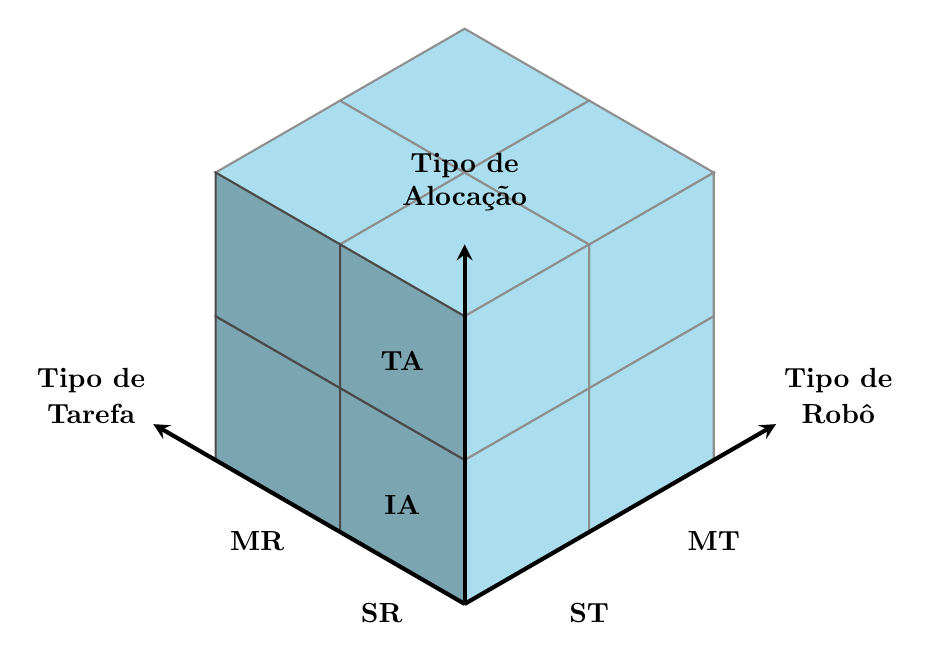
\begin{tikzpicture}
\pgftransformxscale{1.000000}
\pgftransformyscale{-1.000000}
\definecolor{dialinecolor}{rgb}{0.000000, 0.000000, 0.000000}
\pgfsetstrokecolor{dialinecolor}
\definecolor{dialinecolor}{rgb}{1.000000, 1.000000, 1.000000}
\pgfsetfillcolor{dialinecolor}
\pgfsetlinewidth{0.050000\du}
\pgfsetdash{}{0pt}
\pgfsetdash{}{0pt}
\pgfsetmiterjoin
\pgfsetbuttcap
\definecolor{dialinecolor}{rgb}{0.666667, 0.870588, 0.937255}
\pgfsetfillcolor{dialinecolor}
\fill (-5.500000\du,-10.392300\du)--(-2.500000\du,-8.660250\du)--(0.500000\du,-10.392300\du)--(-2.500000\du,-12.124400\du)--cycle;
\definecolor{dialinecolor}{rgb}{0.556863, 0.556863, 0.556863}
\pgfsetstrokecolor{dialinecolor}
\draw (-5.500000\du,-10.392300\du)--(-2.500000\du,-8.660250\du)--(0.500000\du,-10.392300\du)--(-2.500000\du,-12.124400\du)--cycle;
\pgfsetlinewidth{0.050000\du}
\pgfsetdash{}{0pt}
\pgfsetdash{}{0pt}
\pgfsetmiterjoin
\pgfsetbuttcap
\definecolor{dialinecolor}{rgb}{0.666667, 0.870588, 0.937255}
\pgfsetfillcolor{dialinecolor}
\fill (-2.500000\du,-12.124400\du)--(0.500000\du,-10.392300\du)--(3.500000\du,-12.124400\du)--(0.500000\du,-13.856400\du)--cycle;
\definecolor{dialinecolor}{rgb}{0.556863, 0.556863, 0.556863}
\pgfsetstrokecolor{dialinecolor}
\draw (-2.500000\du,-12.124400\du)--(0.500000\du,-10.392300\du)--(3.500000\du,-12.124400\du)--(0.500000\du,-13.856400\du)--cycle;
\pgfsetlinewidth{0.050000\du}
\pgfsetdash{}{0pt}
\pgfsetdash{}{0pt}
\pgfsetmiterjoin
\pgfsetbuttcap
\definecolor{dialinecolor}{rgb}{0.666667, 0.870588, 0.937255}
\pgfsetfillcolor{dialinecolor}
\fill (3.500000\du,-8.660250\du)--(3.500000\du,-5.196150\du)--(6.500000\du,-6.928200\du)--(6.500000\du,-10.392300\du)--cycle;
\definecolor{dialinecolor}{rgb}{0.556863, 0.556863, 0.556863}
\pgfsetstrokecolor{dialinecolor}
\draw (3.500000\du,-8.660250\du)--(3.500000\du,-5.196150\du)--(6.500000\du,-6.928200\du)--(6.500000\du,-10.392300\du)--cycle;
\pgfsetlinewidth{0.050000\du}
\pgfsetdash{}{0pt}
\pgfsetdash{}{0pt}
\pgfsetmiterjoin
\pgfsetbuttcap
\definecolor{dialinecolor}{rgb}{0.666667, 0.870588, 0.937255}
\pgfsetfillcolor{dialinecolor}
\fill (-2.500000\du,-8.660250\du)--(0.500000\du,-6.928200\du)--(3.500000\du,-8.660250\du)--(0.500000\du,-10.392300\du)--cycle;
\definecolor{dialinecolor}{rgb}{0.556863, 0.556863, 0.556863}
\pgfsetstrokecolor{dialinecolor}
\draw (-2.500000\du,-8.660250\du)--(0.500000\du,-6.928200\du)--(3.500000\du,-8.660250\du)--(0.500000\du,-10.392300\du)--cycle;
\pgfsetlinewidth{0.050000\du}
\pgfsetdash{}{0pt}
\pgfsetdash{}{0pt}
\pgfsetmiterjoin
\pgfsetbuttcap
\definecolor{dialinecolor}{rgb}{0.666667, 0.870588, 0.937255}
\pgfsetfillcolor{dialinecolor}
\fill (0.500000\du,-10.392300\du)--(3.500000\du,-8.660250\du)--(6.500000\du,-10.392300\du)--(3.500000\du,-12.124400\du)--cycle;
\definecolor{dialinecolor}{rgb}{0.556863, 0.556863, 0.556863}
\pgfsetstrokecolor{dialinecolor}
\draw (0.500000\du,-10.392300\du)--(3.500000\du,-8.660250\du)--(6.500000\du,-10.392300\du)--(3.500000\du,-12.124400\du)--cycle;
\pgfsetlinewidth{0.050000\du}
\pgfsetdash{}{0pt}
\pgfsetdash{}{0pt}
\pgfsetmiterjoin
\pgfsetbuttcap
\definecolor{dialinecolor}{rgb}{0.666667, 0.870588, 0.937255}
\pgfsetfillcolor{dialinecolor}
\fill (0.500000\du,-6.928200\du)--(0.500000\du,-3.464100\du)--(3.500000\du,-5.196150\du)--(3.500000\du,-8.660250\du)--cycle;
\definecolor{dialinecolor}{rgb}{0.556863, 0.556863, 0.556863}
\pgfsetstrokecolor{dialinecolor}
\draw (0.500000\du,-6.928200\du)--(0.500000\du,-3.464100\du)--(3.500000\du,-5.196150\du)--(3.500000\du,-8.660250\du)--cycle;
\pgfsetlinewidth{0.050000\du}
\pgfsetdash{}{0pt}
\pgfsetdash{}{0pt}
\pgfsetmiterjoin
\pgfsetbuttcap
\definecolor{dialinecolor}{rgb}{0.666667, 0.870588, 0.937255}
\pgfsetfillcolor{dialinecolor}
\fill (0.500000\du,-3.464100\du)--(0.500000\du,0.000000\du)--(3.500000\du,-1.732050\du)--(3.500000\du,-5.196150\du)--cycle;
\definecolor{dialinecolor}{rgb}{0.556863, 0.556863, 0.556863}
\pgfsetstrokecolor{dialinecolor}
\draw (0.500000\du,-3.464100\du)--(0.500000\du,0.000000\du)--(3.500000\du,-1.732050\du)--(3.500000\du,-5.196150\du)--cycle;
\pgfsetlinewidth{0.050000\du}
\pgfsetdash{}{0pt}
\pgfsetdash{}{0pt}
\pgfsetmiterjoin
\pgfsetbuttcap
\definecolor{dialinecolor}{rgb}{0.666667, 0.870588, 0.937255}
\pgfsetfillcolor{dialinecolor}
\fill (3.500000\du,-5.196150\du)--(3.500000\du,-1.732050\du)--(6.500000\du,-3.464100\du)--(6.500000\du,-6.928200\du)--cycle;
\definecolor{dialinecolor}{rgb}{0.556863, 0.556863, 0.556863}
\pgfsetstrokecolor{dialinecolor}
\draw (3.500000\du,-5.196150\du)--(3.500000\du,-1.732050\du)--(6.500000\du,-3.464100\du)--(6.500000\du,-6.928200\du)--cycle;
\pgfsetlinewidth{0.050000\du}
\pgfsetdash{}{0pt}
\pgfsetdash{}{0pt}
\pgfsetmiterjoin
\pgfsetbuttcap
\definecolor{dialinecolor}{rgb}{0.486275, 0.647059, 0.698039}
\pgfsetfillcolor{dialinecolor}
\fill (-2.500000\du,-8.660250\du)--(-2.500000\du,-5.196150\du)--(-5.500000\du,-6.928200\du)--(-5.500000\du,-10.392300\du)--cycle;
\definecolor{dialinecolor}{rgb}{0.290196, 0.290196, 0.290196}
\pgfsetstrokecolor{dialinecolor}
\draw (-2.500000\du,-8.660250\du)--(-2.500000\du,-5.196150\du)--(-5.500000\du,-6.928200\du)--(-5.500000\du,-10.392300\du)--cycle;
\pgfsetlinewidth{0.050000\du}
\pgfsetdash{}{0pt}
\pgfsetdash{}{0pt}
\pgfsetmiterjoin
\pgfsetbuttcap
\definecolor{dialinecolor}{rgb}{0.486275, 0.647059, 0.698039}
\pgfsetfillcolor{dialinecolor}
\fill (0.500000\du,-6.928200\du)--(0.500000\du,-3.464100\du)--(-2.500000\du,-5.196150\du)--(-2.500000\du,-8.660250\du)--cycle;
\definecolor{dialinecolor}{rgb}{0.290196, 0.290196, 0.290196}
\pgfsetstrokecolor{dialinecolor}
\draw (0.500000\du,-6.928200\du)--(0.500000\du,-3.464100\du)--(-2.500000\du,-5.196150\du)--(-2.500000\du,-8.660250\du)--cycle;
\pgfsetlinewidth{0.050000\du}
\pgfsetdash{}{0pt}
\pgfsetdash{}{0pt}
\pgfsetmiterjoin
\pgfsetbuttcap
\definecolor{dialinecolor}{rgb}{0.486275, 0.647059, 0.698039}
\pgfsetfillcolor{dialinecolor}
\fill (-2.500000\du,-5.196150\du)--(-2.500000\du,-1.732050\du)--(-5.500000\du,-3.464100\du)--(-5.500000\du,-6.928200\du)--cycle;
\definecolor{dialinecolor}{rgb}{0.290196, 0.290196, 0.290196}
\pgfsetstrokecolor{dialinecolor}
\draw (-2.500000\du,-5.196150\du)--(-2.500000\du,-1.732050\du)--(-5.500000\du,-3.464100\du)--(-5.500000\du,-6.928200\du)--cycle;
\pgfsetlinewidth{0.050000\du}
\pgfsetdash{}{0pt}
\pgfsetdash{}{0pt}
\pgfsetmiterjoin
\pgfsetbuttcap
\definecolor{dialinecolor}{rgb}{0.486275, 0.647059, 0.698039}
\pgfsetfillcolor{dialinecolor}
\fill (0.500000\du,-3.464100\du)--(0.500000\du,0.000000\du)--(-2.500000\du,-1.732050\du)--(-2.500000\du,-5.196150\du)--cycle;
\definecolor{dialinecolor}{rgb}{0.290196, 0.290196, 0.290196}
\pgfsetstrokecolor{dialinecolor}
\draw (0.500000\du,-3.464100\du)--(0.500000\du,0.000000\du)--(-2.500000\du,-1.732050\du)--(-2.500000\du,-5.196150\du)--cycle;
% setfont left to latex
\definecolor{dialinecolor}{rgb}{0.000000, 0.000000, 0.000000}
\pgfsetstrokecolor{dialinecolor}
\node at (-8.500000\du,-5.374900\du){\textbf{Tipo de}};
% setfont left to latex
\definecolor{dialinecolor}{rgb}{0.000000, 0.000000, 0.000000}
\pgfsetstrokecolor{dialinecolor}
\node at (-8.500000\du,-4.574900\du){\textbf{Tarefa}};
% setfont left to latex
\definecolor{dialinecolor}{rgb}{0.000000, 0.000000, 0.000000}
\pgfsetstrokecolor{dialinecolor}
\node at (0.500000\du,-10.571050\du){\textbf{Tipo de}};
% setfont left to latex
\definecolor{dialinecolor}{rgb}{0.000000, 0.000000, 0.000000}
\pgfsetstrokecolor{dialinecolor}
\node at (0.500000\du,-9.771050\du){\textbf{Alocação}};
% setfont left to latex
\definecolor{dialinecolor}{rgb}{0.000000, 0.000000, 0.000000}
\pgfsetstrokecolor{dialinecolor}
\node at (9.500000\du,-5.374900\du){\textbf{Tipo de}};
% setfont left to latex
\definecolor{dialinecolor}{rgb}{0.000000, 0.000000, 0.000000}
\pgfsetstrokecolor{dialinecolor}
\node at (9.500000\du,-4.574900\du){\textbf{Robô}};
\pgfsetlinewidth{0.100000\du}
\pgfsetdash{}{0pt}
\pgfsetdash{}{0pt}
\pgfsetbuttcap
{
\definecolor{dialinecolor}{rgb}{0.000000, 0.000000, 0.000000}
\pgfsetfillcolor{dialinecolor}
% was here!!!
\pgfsetarrowsstart{stealth}
\definecolor{dialinecolor}{rgb}{0.000000, 0.000000, 0.000000}
\pgfsetstrokecolor{dialinecolor}
\draw (8.000000\du,-4.330130\du)--(0.500000\du,0.000000\du);
}
\pgfsetlinewidth{0.100000\du}
\pgfsetdash{}{0pt}
\pgfsetdash{}{0pt}
\pgfsetbuttcap
{
\definecolor{dialinecolor}{rgb}{0.000000, 0.000000, 0.000000}
\pgfsetfillcolor{dialinecolor}
% was here!!!
\pgfsetarrowsstart{stealth}
\definecolor{dialinecolor}{rgb}{0.000000, 0.000000, 0.000000}
\pgfsetstrokecolor{dialinecolor}
\draw (-7.000000\du,-4.330130\du)--(0.500000\du,0.000000\du);
}
% setfont left to latex
\definecolor{dialinecolor}{rgb}{0.000000, 0.000000, 0.000000}
\pgfsetstrokecolor{dialinecolor}
\node at (-4.500000\du,-1.510800\du){\textbf{MR}};
% setfont left to latex
\definecolor{dialinecolor}{rgb}{0.000000, 0.000000, 0.000000}
\pgfsetstrokecolor{dialinecolor}
\node at (-1.500000\du,0.221250\du){\textbf{SR}};
% setfont left to latex
\definecolor{dialinecolor}{rgb}{0.000000, 0.000000, 0.000000}
\pgfsetstrokecolor{dialinecolor}
\node at (3.500000\du,0.221250\du){\textbf{ST}};
% setfont left to latex
\definecolor{dialinecolor}{rgb}{0.000000, 0.000000, 0.000000}
\pgfsetstrokecolor{dialinecolor}
\node at (6.500000\du,-1.510800\du){\textbf{MT}};
% setfont left to latex
\definecolor{dialinecolor}{rgb}{0.000000, 0.000000, 0.000000}
\pgfsetstrokecolor{dialinecolor}
\node at (-1.000000\du,-5.840930\du){\textbf{TA}};
% setfont left to latex
\definecolor{dialinecolor}{rgb}{0.000000, 0.000000, 0.000000}
\pgfsetstrokecolor{dialinecolor}
\node at (-1.000000\du,-2.376830\du){\textbf{IA}};
\pgfsetlinewidth{0.100000\du}
\pgfsetdash{}{0pt}
\pgfsetdash{}{0pt}
\pgfsetbuttcap
{
\definecolor{dialinecolor}{rgb}{0.000000, 0.000000, 0.000000}
\pgfsetfillcolor{dialinecolor}
% was here!!!
\pgfsetarrowsstart{stealth}
\definecolor{dialinecolor}{rgb}{0.000000, 0.000000, 0.000000}
\pgfsetstrokecolor{dialinecolor}
\draw (0.500000\du,-8.660250\du)--(0.500000\du,0.000000\du);
}
\end{tikzpicture}
